% Options for packages loaded elsewhere
\PassOptionsToPackage{unicode}{hyperref}
\PassOptionsToPackage{hyphens}{url}
\documentclass[
]{article}
\usepackage{xcolor}
\usepackage[margin=1in]{geometry}
\usepackage{amsmath,amssymb}
\setcounter{secnumdepth}{5}
\usepackage{iftex}
\ifPDFTeX
  \usepackage[T1]{fontenc}
  \usepackage[utf8]{inputenc}
  \usepackage{textcomp} % provide euro and other symbols
\else % if luatex or xetex
  \usepackage{unicode-math} % this also loads fontspec
  \defaultfontfeatures{Scale=MatchLowercase}
  \defaultfontfeatures[\rmfamily]{Ligatures=TeX,Scale=1}
\fi
\usepackage{lmodern}
\ifPDFTeX\else
  % xetex/luatex font selection
\fi
% Use upquote if available, for straight quotes in verbatim environments
\IfFileExists{upquote.sty}{\usepackage{upquote}}{}
\IfFileExists{microtype.sty}{% use microtype if available
  \usepackage[]{microtype}
  \UseMicrotypeSet[protrusion]{basicmath} % disable protrusion for tt fonts
}{}
\makeatletter
\@ifundefined{KOMAClassName}{% if non-KOMA class
  \IfFileExists{parskip.sty}{%
    \usepackage{parskip}
  }{% else
    \setlength{\parindent}{0pt}
    \setlength{\parskip}{6pt plus 2pt minus 1pt}}
}{% if KOMA class
  \KOMAoptions{parskip=half}}
\makeatother
\usepackage{color}
\usepackage{fancyvrb}
\newcommand{\VerbBar}{|}
\newcommand{\VERB}{\Verb[commandchars=\\\{\}]}
\DefineVerbatimEnvironment{Highlighting}{Verbatim}{commandchars=\\\{\}}
% Add ',fontsize=\small' for more characters per line
\usepackage{framed}
\definecolor{shadecolor}{RGB}{248,248,248}
\newenvironment{Shaded}{\begin{snugshade}}{\end{snugshade}}
\newcommand{\AlertTok}[1]{\textcolor[rgb]{0.94,0.16,0.16}{#1}}
\newcommand{\AnnotationTok}[1]{\textcolor[rgb]{0.56,0.35,0.01}{\textbf{\textit{#1}}}}
\newcommand{\AttributeTok}[1]{\textcolor[rgb]{0.13,0.29,0.53}{#1}}
\newcommand{\BaseNTok}[1]{\textcolor[rgb]{0.00,0.00,0.81}{#1}}
\newcommand{\BuiltInTok}[1]{#1}
\newcommand{\CharTok}[1]{\textcolor[rgb]{0.31,0.60,0.02}{#1}}
\newcommand{\CommentTok}[1]{\textcolor[rgb]{0.56,0.35,0.01}{\textit{#1}}}
\newcommand{\CommentVarTok}[1]{\textcolor[rgb]{0.56,0.35,0.01}{\textbf{\textit{#1}}}}
\newcommand{\ConstantTok}[1]{\textcolor[rgb]{0.56,0.35,0.01}{#1}}
\newcommand{\ControlFlowTok}[1]{\textcolor[rgb]{0.13,0.29,0.53}{\textbf{#1}}}
\newcommand{\DataTypeTok}[1]{\textcolor[rgb]{0.13,0.29,0.53}{#1}}
\newcommand{\DecValTok}[1]{\textcolor[rgb]{0.00,0.00,0.81}{#1}}
\newcommand{\DocumentationTok}[1]{\textcolor[rgb]{0.56,0.35,0.01}{\textbf{\textit{#1}}}}
\newcommand{\ErrorTok}[1]{\textcolor[rgb]{0.64,0.00,0.00}{\textbf{#1}}}
\newcommand{\ExtensionTok}[1]{#1}
\newcommand{\FloatTok}[1]{\textcolor[rgb]{0.00,0.00,0.81}{#1}}
\newcommand{\FunctionTok}[1]{\textcolor[rgb]{0.13,0.29,0.53}{\textbf{#1}}}
\newcommand{\ImportTok}[1]{#1}
\newcommand{\InformationTok}[1]{\textcolor[rgb]{0.56,0.35,0.01}{\textbf{\textit{#1}}}}
\newcommand{\KeywordTok}[1]{\textcolor[rgb]{0.13,0.29,0.53}{\textbf{#1}}}
\newcommand{\NormalTok}[1]{#1}
\newcommand{\OperatorTok}[1]{\textcolor[rgb]{0.81,0.36,0.00}{\textbf{#1}}}
\newcommand{\OtherTok}[1]{\textcolor[rgb]{0.56,0.35,0.01}{#1}}
\newcommand{\PreprocessorTok}[1]{\textcolor[rgb]{0.56,0.35,0.01}{\textit{#1}}}
\newcommand{\RegionMarkerTok}[1]{#1}
\newcommand{\SpecialCharTok}[1]{\textcolor[rgb]{0.81,0.36,0.00}{\textbf{#1}}}
\newcommand{\SpecialStringTok}[1]{\textcolor[rgb]{0.31,0.60,0.02}{#1}}
\newcommand{\StringTok}[1]{\textcolor[rgb]{0.31,0.60,0.02}{#1}}
\newcommand{\VariableTok}[1]{\textcolor[rgb]{0.00,0.00,0.00}{#1}}
\newcommand{\VerbatimStringTok}[1]{\textcolor[rgb]{0.31,0.60,0.02}{#1}}
\newcommand{\WarningTok}[1]{\textcolor[rgb]{0.56,0.35,0.01}{\textbf{\textit{#1}}}}
\usepackage{graphicx}
\makeatletter
\newsavebox\pandoc@box
\newcommand*\pandocbounded[1]{% scales image to fit in text height/width
  \sbox\pandoc@box{#1}%
  \Gscale@div\@tempa{\textheight}{\dimexpr\ht\pandoc@box+\dp\pandoc@box\relax}%
  \Gscale@div\@tempb{\linewidth}{\wd\pandoc@box}%
  \ifdim\@tempb\p@<\@tempa\p@\let\@tempa\@tempb\fi% select the smaller of both
  \ifdim\@tempa\p@<\p@\scalebox{\@tempa}{\usebox\pandoc@box}%
  \else\usebox{\pandoc@box}%
  \fi%
}
% Set default figure placement to htbp
\def\fps@figure{htbp}
\makeatother
\setlength{\emergencystretch}{3em} % prevent overfull lines
\providecommand{\tightlist}{%
  \setlength{\itemsep}{0pt}\setlength{\parskip}{0pt}}
\setcounter{section}{-1}
\usepackage{fvextra}
\DefineVerbatimEnvironment{Highlighting}{Verbatim}{
  showspaces = false,
  showtabs = false,
  breaklines,
  commandchars=\\\{\}
}

\usepackage{bookmark}
\IfFileExists{xurl.sty}{\usepackage{xurl}}{} % add URL line breaks if available
\urlstyle{same}
% fallback for those not using the hyperref driver hyperxmp:
\makeatletter
\@ifundefined{xmpquote}{\newcommand{\xmpquote}[1]{#1}}{}
\makeatother
\hypersetup{
  pdftitle={QRM II Graded Assignment (14)},
  pdfauthor={group 29: Thea von Sydow, Loek van Wijk, Thomas Dop, Anastasios Goudras and Tim de Marez Oyens},
  hidelinks,
  pdfcreator={LaTeX via pandoc}}

\title{QRM II Graded Assignment (14)}
\usepackage{etoolbox}
\makeatletter
\providecommand{\subtitle}[1]{% add subtitle to \maketitle
  \apptocmd{\@title}{\par {\large #1 \par}}{}{}
}
\makeatother
\subtitle{Period 1, 2026}
\author{group 29: Thea von Sydow, Loek van Wijk, Thomas Dop, Anastasios
Goudras and Tim de Marez Oyens}
\date{25-09-2026}

\begin{document}
\maketitle

\section{Introduction}\label{introduction}

This assignment is to be completed in groups of 4-5. Further, all
students in your group need to be assigned to the same R tutorial group
(Friday's tutorial). You can sign yourself up for a group on Canvas.
Please do so
\textbf{before the start of your first R tutorial on Friday September 4th.}
You can use the Discussion Board in Canvas if you do not have a group
yet or if your group is incomplete.

The assignment has 5 parts, and each part corresponds to the course
material of that week (with the exclusion of week 6, for which there is
no R programming material).

You are supposed to hand in these assignments on Canvas at the following
dates:

\begin{itemize}
\tightlist
\item
  \textbf{Deadline 1} \emph{Sunday September 27th, at 23:59pm}: you are
  supposed to hand in weeks 1, 2, and 3 of this assignment. This will
  determine 18\% of your overall course grade
\item
  \textbf{Deadline 2} \emph{Sunday October 11th, at 23:59pm}: you are
  supposed to hand in weeks 4, and 5 of this assignment. This will
  determine 12\% of your overall course grade
\end{itemize}

The R tutorials (each Friday) will consist of two halves. During the
first half, you will discuss the tutorial exercises. These can be
downloaded separately from Canvas. During the second half, you can work
on this graded assignment within your own group. The purpose is that you
find out how to work with R for doing statistical analyses by yourself.
The tutorial exercises are meant to teach you basic commands to get you
started, but to answer the problem sets in this assignment, you might
need to research your own solutions, and use functions and commands not
described in the tutorial exercises. Learning how to solve your own
research problems is integral part of learning R. When you and your
group get stuck on how to approach an exercise, the hierarchy in finding
your way is as follows:

\begin{itemize}
\tightlist
\item
  use the concepts from the tutorial exercises;
\item
  use the cheat sheets available on Canvas;
\item
  use Google, YouTube, StackOverflow, or another website;
\item
  ask the teacher.
\end{itemize}

The use of generative AI is \textbf{not} permitted and may result in a
grade of 0. See the AI protocol in the course manual for details.

To answer the assignment, you can simply fill out this R markdown
document. There are designated places which you can fill with R code.
There are also designated spaces for you to answer each question. Often,
the structure of an answer will be as follows. First, you type the R
code in the designated box. This will show how you analyzed the data to
get the answer to the question. Below the box for the R code, you will
then summarize your answer to the question, i.e.~what are the
conclusions that you draw from the data analysis?

When handing in, you are supposed to submit this .Rmd file, and a
knitted version of this document. You can knit this document to pdf,
word, or html. Knitting to pdf requires you to have a .tex distribution
installed on your computer. Knitting to Word requires you to have Word
installed.

The exercises are designed such that you should be able to finish the
majority of them during the tutorial each week. If you are not able to
finish them fully during that time, you are expected to work on it in
your own time using the computers on campus or your own device. It is
best to meet as a group in-person when working together. If you want to
work remotely, github is a good platform to guarantee smooth
collaboration. Alternatively, you can email this .Rmd file back and
forth to one another as a group, but this is not recommended as it is
more cumbersome.

We encourage you to keep your code blocks, printing statements, and
final answers, as short as possible. In any case, there is a page limit
of 6 pages per week, which encompasses the total length of this document
which consists of the questions, your coding lines, and your answers.
When your answers to questions of the respective week exceed this page
limit, they will not be graded, resulting in zero points.

Each week consists of 1, 2, or 3 subquestions. The total amount of
points you can earn per week is 20 points.

\section{Week 1}\label{week-1}

\begin{enumerate}
\def\labelenumi{\arabic{enumi}.}
\tightlist
\item
  Find the dataset ``movies1.tsv'' on Canvas. Describe your data set:
  How many observations does it have. How many variables are there? How
  many subjects? What consists of a subject? \textbf{[4 points]}
\end{enumerate}

\begin{Shaded}
\begin{Highlighting}[]
\FunctionTok{library}\NormalTok{(readr)}
\NormalTok{movies1 }\OtherTok{\textless{}{-}} \FunctionTok{read\_tsv}\NormalTok{(}\StringTok{"movies1.tsv"}\NormalTok{)}
\end{Highlighting}
\end{Shaded}

\begin{verbatim}
## Rows: 505 Columns: 19
## -- Column specification --------------------------------------------------------
## Delimiter: "\t"
## chr   (8): keywords, original_language, title, genre, first_actor, first_act...
## dbl  (10): index, budget, popularity, revenue, runtime, vote_average, vote_c...
## date  (1): release_date
## 
## i Use `spec()` to retrieve the full column specification for this data.
## i Specify the column types or set `show_col_types = FALSE` to quiet this message.
\end{verbatim}

\begin{Shaded}
\begin{Highlighting}[]
\FunctionTok{nrow}\NormalTok{(movies1)}
\end{Highlighting}
\end{Shaded}

\begin{verbatim}
## [1] 505
\end{verbatim}

\begin{Shaded}
\begin{Highlighting}[]
\FunctionTok{ncol}\NormalTok{(movies1)}
\end{Highlighting}
\end{Shaded}

\begin{verbatim}
## [1] 19
\end{verbatim}

\textbf{Your Answer:}

Write your response here. it has 19 variables it has 505 subjects it has

\begin{enumerate}
\def\labelenumi{\arabic{enumi}.}
\setcounter{enumi}{1}
\tightlist
\item
  Which of the following types of variables are present in your data
  set? (i) nominal; (ii) ordinal; (iii); interval; (iv) ratio. If
  present, name one example of such a variable present in your data set.
  \textbf{[4 points]}
\end{enumerate}

\begin{Shaded}
\begin{Highlighting}[]
\FunctionTok{str}\NormalTok{(movies1)}
\end{Highlighting}
\end{Shaded}

\begin{verbatim}
## spc_tbl_ [505 x 19] (S3: spec_tbl_df/tbl_df/tbl/data.frame)
##  $ index              : num [1:505] 1773 2540 1174 3262 4324 ...
##  $ budget             : num [1:505] 2.70e+07 1.50e+07 4.00e+07 0.00 0.00 1.20e+08 2.80e+07 7.00e+07 1.25e+07 4.00e+07 ...
##  $ keywords           : chr [1:505] "fbi island serial killer series of murders" "fire winter santa claus snow storm christmas tree" "police sequel police officer brother-in-law brother-in-law relationship black men" "masseuse thanksgiving party romance mother daughter relationship" ...
##  $ original_language  : chr [1:505] "en" "en" "en" "en" ...
##  $ title              : chr [1:505] "Mindhunters" "Krampus" "Ride Along 2" "Enough Said" ...
##  $ popularity         : num [1:505] 17.194 31.565 25.136 14.969 0.148 ...
##  $ release_date       : Date[1:505], format: "2004-05-07" "2015-11-26" ...
##  $ revenue            : num [1:505] 2.11e+07 6.15e+07 1.25e+08 2.53e+07 0.00 ...
##  $ runtime            : num [1:505] 106 98 102 93 97 130 108 99 100 99 ...
##  $ vote_average       : num [1:505] 6.3 5.9 6.1 6.6 6 6.2 5.5 4.4 6 6.2 ...
##  $ vote_count         : num [1:505] 333 584 555 348 9 597 640 533 210 371 ...
##  $ genre              : chr [1:505] "Thriller" "Comedy" "Comedy" "Drama" ...
##  $ release_year       : num [1:505] 2004 2015 2016 2013 2006 ...
##  $ release_month      : num [1:505] 5 11 1 9 10 3 2 1 2 9 ...
##  $ release_day        : num [1:505] 7 26 14 18 27 15 4 10 14 29 ...
##  $ first_actor        : chr [1:505] "LL Cool" "Adam Scott" "Kevin Hart" "Julia Louis-Dreyfus" ...
##  $ first_actor_gender : chr [1:505] NA "male" "male" "female" ...
##  $ director_first_name: chr [1:505] "Renny" "Michael" "Tim" "Nicole" ...
##  $ director_gender    : chr [1:505] "male" "male" "male" "female" ...
##  - attr(*, "spec")=
##   .. cols(
##   ..   index = col_double(),
##   ..   budget = col_double(),
##   ..   keywords = col_character(),
##   ..   original_language = col_character(),
##   ..   title = col_character(),
##   ..   popularity = col_double(),
##   ..   release_date = col_date(format = ""),
##   ..   revenue = col_double(),
##   ..   runtime = col_double(),
##   ..   vote_average = col_double(),
##   ..   vote_count = col_double(),
##   ..   genre = col_character(),
##   ..   release_year = col_double(),
##   ..   release_month = col_double(),
##   ..   release_day = col_double(),
##   ..   first_actor = col_character(),
##   ..   first_actor_gender = col_character(),
##   ..   director_first_name = col_character(),
##   ..   director_gender = col_character()
##   .. )
##  - attr(*, "problems")=<pointer: 0x0000019fbeaffd50>
\end{verbatim}

\begin{Shaded}
\begin{Highlighting}[]
\FunctionTok{summary}\NormalTok{(movies1)}
\end{Highlighting}
\end{Shaded}

\begin{verbatim}
##      index          budget               keywords   original_language
##  Min.   :   0   Min.   :        0   Length   :505   Length   :505    
##  1st Qu.:1056   1st Qu.:        0   N.unique :447   N.unique : 13    
##  Median :2283   Median : 15000000   N.blank  :  0   N.blank  :  0    
##  Mean   :2335   Mean   : 31694006   Min.nchar:  3   Min.nchar:  2    
##  3rd Qu.:3581   3rd Qu.: 45000000   Max.nchar:129   Max.nchar:  2    
##  Max.   :4796   Max.   :250000000   NAs      : 53                    
##                                                                      
##        title       popularity         release_date           revenue         
##  Length   :505   Min.   :2.386e-03   Min.   :1990-01-19   Min.   :0.000e+00  
##  N.unique :505   1st Qu.:4.759e+00   1st Qu.:2002-04-12   1st Qu.:0.000e+00  
##  N.blank  :  0   Median :1.414e+01   Median :2007-06-01   Median :1.948e+07  
##  Min.nchar:  3   Mean   :2.283e+01   Mean   :2006-11-25   Mean   :9.482e+07  
##  Max.nchar: 62   3rd Qu.:2.985e+01   3rd Qu.:2012-05-25   3rd Qu.:1.043e+08  
##                  Max.   :2.037e+02   Max.   :2016-08-02   Max.   :2.788e+09  
##                                                                              
##     runtime     vote_average     vote_count            genre      release_year 
##  Min.   :  0   Min.   :0.000   Min.   :    0.0   Length   :505   Min.   :1990  
##  1st Qu.: 94   1st Qu.:5.600   1st Qu.:   47.0   N.unique : 13   1st Qu.:2002  
##  Median :103   Median :6.200   Median :  255.0   N.blank  :  0   Median :2007  
##  Mean   :107   Mean   :6.043   Mean   :  802.9   Min.nchar:  5   Mean   :2006  
##  3rd Qu.:118   3rd Qu.:6.800   3rd Qu.:  914.0   Max.nchar: 11   3rd Qu.:2012  
##  Max.   :276   Max.   :8.100   Max.   :11800.0   NAs      :  5   Max.   :2016  
##  NAs    :1                                                                     
##  release_month     release_day       first_actor  first_actor_gender
##  Min.   : 1.000   Min.   : 1.00   Length   :505   Length   :505     
##  1st Qu.: 4.000   1st Qu.: 8.00   N.unique :405   N.unique :  2     
##  Median : 8.000   Median :15.00   N.blank  :  0   N.blank  :  0     
##  Mean   : 6.968   Mean   :15.29   Min.nchar:  6   Min.nchar:  4     
##  3rd Qu.:10.000   3rd Qu.:23.00   Max.nchar: 23   Max.nchar:  6     
##  Max.   :12.000   Max.   :31.00   NAs      :  8   NAs      : 23     
##                                                                     
##  director_first_name  director_gender
##  Length   :505       Length   :505   
##  N.unique :266       N.unique :  2   
##  N.blank  :  0       N.blank  :  0   
##  Min.nchar:  2       Min.nchar:  4   
##  Max.nchar: 14       Max.nchar:  6   
##  NAs      :  6       NAs      : 35   
## 
\end{verbatim}

\begin{Shaded}
\begin{Highlighting}[]
\FunctionTok{head}\NormalTok{(movies1)}
\end{Highlighting}
\end{Shaded}

\begin{verbatim}
## # A tibble: 6 x 19
##   index  budget keywords original_language title popularity release_date revenue
##   <dbl>   <dbl> <chr>    <chr>             <chr>      <dbl> <date>         <dbl>
## 1  1773  2.70e7 fbi isl~ en                Mind~     17.2   2004-05-07    2.11e7
## 2  2540  1.5 e7 fire wi~ en                Kram~     31.6   2015-11-26    6.15e7
## 3  1174  4   e7 police ~ en                Ride~     25.1   2016-01-14    1.25e8
## 4  3262  0      masseus~ en                Enou~     15.0   2013-09-18    2.53e7
## 5  4324  0      christi~ en                Fait~      0.148 2006-10-27    0     
## 6   214  1.20e8 u.s. ai~ en                The ~     25.8   2000-03-15    3.26e8
## # i 11 more variables: runtime <dbl>, vote_average <dbl>, vote_count <dbl>,
## #   genre <chr>, release_year <dbl>, release_month <dbl>, release_day <dbl>,
## #   first_actor <chr>, first_actor_gender <chr>, director_first_name <chr>,
## #   director_gender <chr>
\end{verbatim}

\textbf{Your Answer:}

Write your response here. All four data types are present Nominal -
genre ordinal - release\_month interval - release\_date ratio - budget

\begin{enumerate}
\def\labelenumi{\arabic{enumi}.}
\setcounter{enumi}{2}
\tightlist
\item
  A movie studio wants to know which types of movies give maximal
  profit. Perform the following steps to provide the movie studio with
  an analysis which corresponds to their request:
\end{enumerate}

\begin{enumerate}
\def\labelenumi{\alph{enumi}.}
\item
  Create the variable profits as the revenue of a movie minus its
  budget. Report its mean, median, maximum, and minimum.
  \textbf{[2 points]}
\item
  Which movie has the highest profits in your data set and how much are
  these profits. Which movie has the lowest and how much are its
  profits? If multiple movies have the exact same highest or lowest
  profits, give only one example. \textbf{[2 points]}
\item
  Create a boxplot of the variable profits. Make sure it has an
  appropriate title, and appropriate titles and labels for the x- and
  y-axis. Give Q1, Q2, Q3, and Q4. What does this tell you about the
  nature of making money in the movies industry? \textbf{[2 points]}
\item
  Add a new variable to your data set the log of profits. When creating
  this variable, what happens to movies for which profits is zero or
  negative? What then happens when you calculate the mean of log of
  profits? \textbf{[2 points]}
\item
  For movies that have a profit of zero or less, replace log of profits
  with ``NA''. What is now the mean of log of profits? Create a boxplot
  for log of profits, again with an appropriate title, x- and y-axis
  labels. How does it compare to the boxplot you made under c.)?
  \textbf{[2 points]}
\item
  Create a scatterplot of with the runtime of movies on the x-axis and
  the average vote of movies on the y-axis. What do you conclude from
  the scatterplot? Are movies with a longer runtime considered worse or
  better by the audience, or does the audience not have a preference?
  Why do you think this is the case? \textbf{[2 points]}
\end{enumerate}

For each step, you should provide first all the code you used to answer
the question and then formulate an answer using full sentences.

\emph{Step a}

\begin{Shaded}
\begin{Highlighting}[]
\FunctionTok{library}\NormalTok{(readr)}

\NormalTok{movies1 }\OtherTok{\textless{}{-}} \FunctionTok{read\_tsv}\NormalTok{(}\StringTok{"movies1.tsv"}\NormalTok{, }\AttributeTok{show\_col\_types =} \ConstantTok{FALSE}\NormalTok{)}

\NormalTok{movies1}\SpecialCharTok{$}\NormalTok{profits }\OtherTok{\textless{}{-}}\NormalTok{ movies1}\SpecialCharTok{$}\NormalTok{revenue }\SpecialCharTok{{-}}\NormalTok{ movies1}\SpecialCharTok{$}\NormalTok{budget}

\FunctionTok{mean}\NormalTok{(movies1}\SpecialCharTok{$}\NormalTok{profits)}
\end{Highlighting}
\end{Shaded}

\begin{verbatim}
## [1] 63121475
\end{verbatim}

\begin{Shaded}
\begin{Highlighting}[]
\FunctionTok{median}\NormalTok{(movies1}\SpecialCharTok{$}\NormalTok{profits)}
\end{Highlighting}
\end{Shaded}

\begin{verbatim}
## [1] 1900000
\end{verbatim}

\begin{Shaded}
\begin{Highlighting}[]
\FunctionTok{max}\NormalTok{(movies1}\SpecialCharTok{$}\NormalTok{profits)}
\end{Highlighting}
\end{Shaded}

\begin{verbatim}
## [1] 2550965087
\end{verbatim}

\begin{Shaded}
\begin{Highlighting}[]
\FunctionTok{min}\NormalTok{(movies1}\SpecialCharTok{$}\NormalTok{profits)}
\end{Highlighting}
\end{Shaded}

\begin{verbatim}
## [1] -9e+07
\end{verbatim}

**Your Answer: After creating profits as revenue minus budget, the
average profit across the 505 movies is \$63,121,475, but the median is
only \$1,900,000. Profits range from a low of -\$90,000,000 (a loss) up
to a high of \$2,550,965,087. The big gap between the mean and median
already suggests the data is skewed, since a few really successful
movies are dragging the average up while most movies make much less.

\emph{Step b}

\begin{Shaded}
\begin{Highlighting}[]
\NormalTok{movies1}\SpecialCharTok{$}\NormalTok{profit }\OtherTok{\textless{}{-}}\NormalTok{ movies1}\SpecialCharTok{$}\NormalTok{revenue }\SpecialCharTok{{-}}\NormalTok{ movies1}\SpecialCharTok{$}\NormalTok{budget}

\NormalTok{highest\_profit\_movie }\OtherTok{\textless{}{-}}\NormalTok{ movies1[}\FunctionTok{which.max}\NormalTok{(movies1}\SpecialCharTok{$}\NormalTok{profit), ]}
\NormalTok{highest\_profit\_movie[, }\FunctionTok{c}\NormalTok{(}\StringTok{"title"}\NormalTok{, }\StringTok{"profit"}\NormalTok{)]}
\end{Highlighting}
\end{Shaded}

\begin{verbatim}
## # A tibble: 1 x 2
##   title      profit
##   <chr>       <dbl>
## 1 Avatar 2550965087
\end{verbatim}

\begin{Shaded}
\begin{Highlighting}[]
\NormalTok{lowest\_profit\_movie }\OtherTok{\textless{}{-}}\NormalTok{ movies1[}\FunctionTok{which.min}\NormalTok{(movies1}\SpecialCharTok{$}\NormalTok{profit), ]}
\NormalTok{lowest\_profit\_movie[, }\FunctionTok{c}\NormalTok{(}\StringTok{"title"}\NormalTok{, }\StringTok{"profit"}\NormalTok{)]}
\end{Highlighting}
\end{Shaded}

\begin{verbatim}
## # A tibble: 1 x 2
##   title               profit
##   <chr>                <dbl>
## 1 Mighty Joe Young -90000000
\end{verbatim}

\textbf{Your Answer:}

The highest profit is Avatar, which has a profit of 2,550,965,087
dollars The lowest profit is Mighty Joe Young, which has a loss of
90,000,000 dollars

\emph{Step c}

\begin{Shaded}
\begin{Highlighting}[]
\FunctionTok{library}\NormalTok{(ggplot2)}
\NormalTok{movies1}\SpecialCharTok{$}\NormalTok{profit }\OtherTok{\textless{}{-}}\NormalTok{ movies1}\SpecialCharTok{$}\NormalTok{revenue }\SpecialCharTok{{-}}\NormalTok{ movies1}\SpecialCharTok{$}\NormalTok{budget}
\FunctionTok{quantile}\NormalTok{(movies1}\SpecialCharTok{$}\NormalTok{profit, }\AttributeTok{na.rm =} \ConstantTok{TRUE}\NormalTok{)}
\end{Highlighting}
\end{Shaded}

\begin{verbatim}
##         0%        25%        50%        75%       100% 
##  -90000000          0    1900000   60514050 2550965087
\end{verbatim}

\begin{Shaded}
\begin{Highlighting}[]
\FunctionTok{ggplot}\NormalTok{(movies1, }\FunctionTok{aes}\NormalTok{(}\AttributeTok{x =} \StringTok{""}\NormalTok{, }\AttributeTok{y =}\NormalTok{ profit)) }\SpecialCharTok{+}
  \FunctionTok{geom\_boxplot}\NormalTok{(}\AttributeTok{fill =} \StringTok{"gray"}\NormalTok{, }\AttributeTok{color =} \StringTok{"black"}\NormalTok{, }\AttributeTok{outlier.color =} \StringTok{"red"}\NormalTok{) }\SpecialCharTok{+}
  \FunctionTok{labs}\NormalTok{(}
    \AttributeTok{title =} \StringTok{"Distribution of Movie Profits"}\NormalTok{,}
    \AttributeTok{x =} \StringTok{"Movies"}\NormalTok{,}
    \AttributeTok{y =} \StringTok{"Profit"}
\NormalTok{  ) }\SpecialCharTok{+}
  \FunctionTok{theme\_minimal}\NormalTok{()}
\end{Highlighting}
\end{Shaded}

\pandocbounded{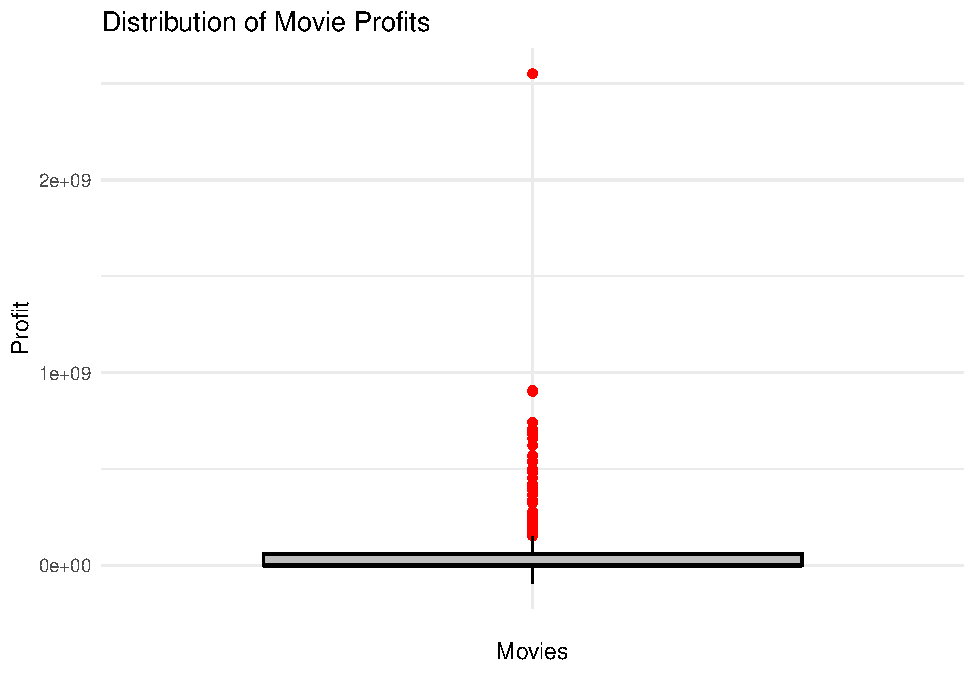
\includegraphics[keepaspectratio]{Assignment14_files/Assignment14_files/figure-latex/unnamed-chunk-5-1.pdf}}

\textbf{Your Answer:} The movie industry is very high risk high reward,
whilst most movies either break even or make a small profit, or a small
loss, only a low amount of movies actually make a large profit

\emph{Step d}

\begin{Shaded}
\begin{Highlighting}[]
\NormalTok{movies1}\SpecialCharTok{$}\NormalTok{logprofits }\OtherTok{\textless{}{-}} \FunctionTok{log}\NormalTok{(movies1}\SpecialCharTok{$}\NormalTok{profits)}
\end{Highlighting}
\end{Shaded}

\begin{verbatim}
## Warning in log(movies1$profits): NaNs produced
\end{verbatim}

\begin{Shaded}
\begin{Highlighting}[]
\FunctionTok{mean}\NormalTok{(movies1}\SpecialCharTok{$}\NormalTok{logprofits)}
\end{Highlighting}
\end{Shaded}

\begin{verbatim}
## [1] NaN
\end{verbatim}

\textbf{Your Answer:}

When we take the log of profits, movies with a profit of exactly zero
end up as -Inf, since the log of zero is undefined and trends toward
negative infinity. Movies with negative profits (losses) turn into NaN,
because you can't take the log of a negative number at all. R even
throws a warning about this, saying ``NaNs produced.'' Since 116 of the
505 movies in the data set have profits of zero or less, all of these
rows get one of these problematic values instead of a real number.

Because of this, when we calculate the mean of logprofits, the result is
NaN. R can't average a column that contains undefined values like NaN
and -Inf alongside normal numbers, so the whole calculation breaks down,
even though most of the individual values are perfectly fine..

\emph{Step e}

\begin{Shaded}
\begin{Highlighting}[]
\NormalTok{movies1}\SpecialCharTok{$}\NormalTok{profit }\OtherTok{\textless{}{-}}\NormalTok{ movies1}\SpecialCharTok{$}\NormalTok{revenue }\SpecialCharTok{{-}}\NormalTok{ movies1}\SpecialCharTok{$}\NormalTok{budget}
\NormalTok{movies1}\SpecialCharTok{$}\NormalTok{log\_profit }\OtherTok{\textless{}{-}} \FunctionTok{log}\NormalTok{(movies1}\SpecialCharTok{$}\NormalTok{profit)}
\end{Highlighting}
\end{Shaded}

\begin{verbatim}
## Warning in log(movies1$profit): NaNs produced
\end{verbatim}

\begin{Shaded}
\begin{Highlighting}[]
\NormalTok{movies1}\SpecialCharTok{$}\NormalTok{log\_profit[movies1}\SpecialCharTok{$}\NormalTok{profit }\SpecialCharTok{\textless{}=} \DecValTok{0}\NormalTok{] }\OtherTok{\textless{}{-}} \ConstantTok{NA}
\NormalTok{mean\_log\_profit }\OtherTok{\textless{}{-}} \FunctionTok{mean}\NormalTok{(movies1}\SpecialCharTok{$}\NormalTok{log\_profit, }\AttributeTok{na.rm =} \ConstantTok{TRUE}\NormalTok{)}
\NormalTok{mean\_log\_profit}
\end{Highlighting}
\end{Shaded}

\begin{verbatim}
## [1] 17.38094
\end{verbatim}

\begin{Shaded}
\begin{Highlighting}[]
\FunctionTok{ggplot}\NormalTok{(movies1[}\SpecialCharTok{!}\FunctionTok{is.na}\NormalTok{(movies1}\SpecialCharTok{$}\NormalTok{log\_profit), ], }\FunctionTok{aes}\NormalTok{(}\AttributeTok{x =} \StringTok{""}\NormalTok{, }\AttributeTok{y =}\NormalTok{ log\_profit)) }\SpecialCharTok{+}
  \FunctionTok{geom\_boxplot}\NormalTok{(}\AttributeTok{fill =} \StringTok{"gray"}\NormalTok{, }\AttributeTok{color =} \StringTok{"black"}\NormalTok{, }\AttributeTok{outlier.color =} \StringTok{"red"}\NormalTok{) }\SpecialCharTok{+}
  \FunctionTok{labs}\NormalTok{(}
    \AttributeTok{title =} \StringTok{"Distribution of log{-}transformed movie profits"}\NormalTok{,}
    \AttributeTok{x =} \StringTok{"Profitable movies"}\NormalTok{,}
    \AttributeTok{y =} \StringTok{"Log of profit"}
\NormalTok{  ) }\SpecialCharTok{+}
  \FunctionTok{theme\_minimal}\NormalTok{()}
\end{Highlighting}
\end{Shaded}

\pandocbounded{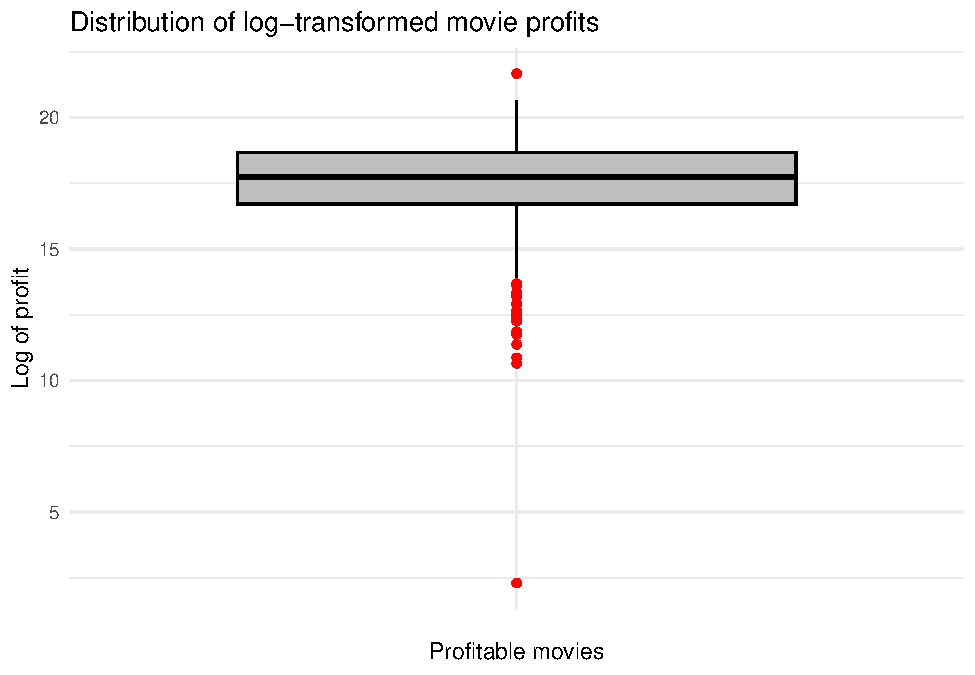
\includegraphics[keepaspectratio]{Assignment14_files/Assignment14_files/figure-latex/unnamed-chunk-7-1.pdf}}

\textbf{Your Answer:}

The boxplot in C had a lot of massive outliers, whilst this one is a bit
more centered arount its median. plus the boxplot in C had a lot more
movies, since we deleted all the once making a loss or breaking even

\emph{Step f}

\begin{Shaded}
\begin{Highlighting}[]
\FunctionTok{plot}\NormalTok{(movies1}\SpecialCharTok{$}\NormalTok{runtime, movies1}\SpecialCharTok{$}\NormalTok{vote\_average,}
     \AttributeTok{main =} \StringTok{"Runtime vs Average Vote"}\NormalTok{,}
     \AttributeTok{xlab =} \StringTok{"Runtime (minutes)"}\NormalTok{,}
     \AttributeTok{ylab =} \StringTok{"Average Vote"}\NormalTok{)}
\end{Highlighting}
\end{Shaded}

\pandocbounded{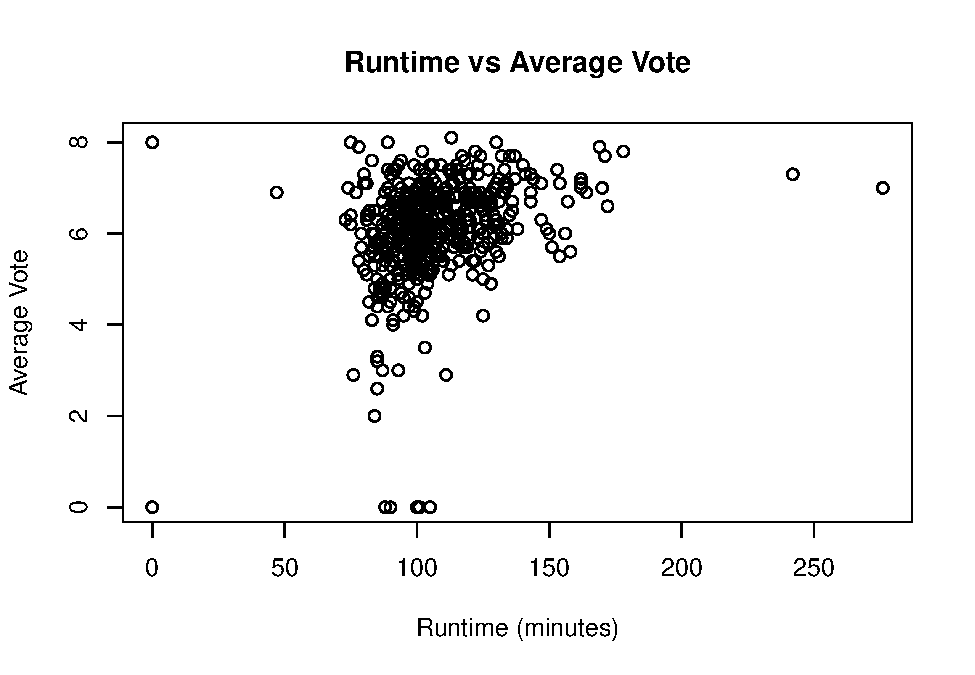
\includegraphics[keepaspectratio]{Assignment14_files/Assignment14_files/figure-latex/unnamed-chunk-8-1.pdf}}

\begin{Shaded}
\begin{Highlighting}[]
\FunctionTok{cor}\NormalTok{(movies1}\SpecialCharTok{$}\NormalTok{runtime, movies1}\SpecialCharTok{$}\NormalTok{vote\_average, }\AttributeTok{use =} \StringTok{"complete.obs"}\NormalTok{)}
\end{Highlighting}
\end{Shaded}

\begin{verbatim}
## [1] 0.3211682
\end{verbatim}

This gives a correlation of about 0.32 between runtime and average vote.
Looking at the scatterplot, most movies cluster between about 90 and 130
minutes with average votes somewhere between 5 and 7.5, and there's a
mild upward trend running through the cloud of points. Longer movies do
tend to get slightly higher ratings on average, but the relationship is
pretty weak, since a correlation of 0.32 means runtime only accounts for
a small part of the variation in how movies get rated. So overall,
audiences seem to have a slight preference for longer movies, but it's
not a strong effect. A likely reason is that longer runtimes often go
along with bigger productions, more developed stories, and higher
budgets, things like epics or dramas that studios invest more time and
money into tend to run longer, and that extra effort may translate into
somewhat better reception.

\section{Week 2}\label{week-2}

1 Is your dataset movies1.tsv the full population, or is it a sample of
a larger population? If the latter, how would you describe the full
population? \textbf{[4 points]}

\textbf{Your Answer:}

It is a sample of a larger population, the full population would include
every single movie made globally, and since this dataset only includes
505 movies, it is a sample.

2 a. For which actor in your data set do you observe the most movies?
\textbf{[2 points]} b. What is the average revenue of the movie in which
this actor plays and does the revenue lie above or below the revenue of
an average movie according to your data set? \textbf{[2 points]}\\
c.~How trustworthy do you consider your conclusion to answer 2b? Use the
term ``law of large numbers'' in your explanation. \textbf{[2 points]}

\emph{step a}

\begin{Shaded}
\begin{Highlighting}[]
\FunctionTok{library}\NormalTok{ (dplyr)}
\end{Highlighting}
\end{Shaded}

\begin{verbatim}
## 
## Attaching package: 'dplyr'
\end{verbatim}

\begin{verbatim}
## The following objects are masked from 'package:stats':
## 
##     filter, lag
\end{verbatim}

\begin{verbatim}
## The following objects are masked from 'package:base':
## 
##     intersect, setdiff, setequal, union
\end{verbatim}

\begin{Shaded}
\begin{Highlighting}[]
\NormalTok{movies1 }\SpecialCharTok{\%\textgreater{}\%}
  \FunctionTok{filter}\NormalTok{(}\SpecialCharTok{!}\FunctionTok{is.na}\NormalTok{(first\_actor)) }\SpecialCharTok{\%\textgreater{}\%}
  \FunctionTok{count}\NormalTok{(first\_actor, }\AttributeTok{sort =} \ConstantTok{TRUE}\NormalTok{) }\SpecialCharTok{\%\textgreater{}\%}
  \FunctionTok{head}\NormalTok{(}\DecValTok{1}\NormalTok{)}
\end{Highlighting}
\end{Shaded}

\begin{verbatim}
## # A tibble: 1 x 2
##   first_actor      n
##   <chr>        <int>
## 1 Bruce Willis     7
\end{verbatim}

\textbf{Your Answer:} The actor with the most movies (in this sample) is
Bruce Willis who has 7 movies (in this sample).

\emph{step b}

\begin{Shaded}
\begin{Highlighting}[]
\NormalTok{movies\_bruce }\OtherTok{\textless{}{-}} \FunctionTok{subset}\NormalTok{(movies1, first\_actor }\SpecialCharTok{==} \StringTok{"Bruce Willis"}\NormalTok{)}
\NormalTok{Average\_revenue\_Bruce }\OtherTok{\textless{}{-}} \FunctionTok{mean}\NormalTok{(movies\_bruce}\SpecialCharTok{$}\NormalTok{revenue, }\AttributeTok{na.rm =} \ConstantTok{TRUE}\NormalTok{)}

\NormalTok{Average\_Revenue }\OtherTok{\textless{}{-}} \FunctionTok{mean}\NormalTok{(movies1}\SpecialCharTok{$}\NormalTok{revenue, }\AttributeTok{na.rm =} \ConstantTok{TRUE}\NormalTok{)}
\end{Highlighting}
\end{Shaded}

\textbf{Your Answer:}

The average revenue for a Bruce Willis film is 116,280,089.57 U.S.
Dollars The average revenue for all the movies is 94,815,481.64 U.S.
Dollars

This means that the average Bruce Willis movie generates more revenue
than the average movie from this sample.

\emph{step c}

\begin{Shaded}
\begin{Highlighting}[]
\CommentTok{\#WRITE YOUR CODE HERE}
\end{Highlighting}
\end{Shaded}

\textbf{Your Answer:}

It is not very trustworthy since this sample is only a small percentage
of all movies made. According to the law of large numbers, the more
movies you add to the sample, the closer you would get to the `true
mean'. And since we are only analyzing 505 movies and 7 Bruce Willis
movies, the possibility is very large that the answer is distorted.
(e.g.~there could be one massive outlier which manipulates the outcome)

3 For this question, you will assume that your data set is the full
population.

\begin{enumerate}
\def\labelenumi{\alph{enumi}.}
\tightlist
\item
  Recode profits such that it is expressed in millions. What is the
  variance of the variable profits (in millions) in your data set?
  \textbf{[2 points]}
\item
  Create a new data set, called movies\_sample. Make sure that it is a
  random sample of your data set of 25 movies. What is the variance of
  profits in this random sample? How does it compare to the variance of
  profits in 2a? \textbf{[2 points]}
\item
  In a for loop, create 100 different samples of 25 movies, as in b, and
  estimate the variance within each sample. Save the variance of each
  sample in a vector called sample\_vars. So the first position of the
  vector would have the variance of the first sample, the second
  position the variance of the second sample, etc. Print the start of
  this vector. \textbf{[2 points]}
\item
  Summarize and make a histogram of sample\_vars. What is the mean,
  standard deviation and shape of its distribution? \textbf{[2 points]}
\item
  In your opinion, is a sample of 25 movies sufficient to get a reliable
  estimate of the population variance of profits, using the sample
  variance? Explain? \textbf{[2 points]}
\end{enumerate}

\emph{step a}

\begin{Shaded}
\begin{Highlighting}[]
\NormalTok{movies1}\SpecialCharTok{$}\NormalTok{profits }\OtherTok{\textless{}{-}}\NormalTok{ movies1}\SpecialCharTok{$}\NormalTok{revenue }\SpecialCharTok{{-}}\NormalTok{ movies1}\SpecialCharTok{$}\NormalTok{budget}
\NormalTok{movies1}\SpecialCharTok{$}\NormalTok{profits\_millions }\OtherTok{\textless{}{-}}\NormalTok{ movies1}\SpecialCharTok{$}\NormalTok{profits }\SpecialCharTok{/} \FloatTok{1e6} 

\NormalTok{n }\OtherTok{\textless{}{-}} \FunctionTok{nrow}\NormalTok{(movies1)}
\NormalTok{pop\_var }\OtherTok{\textless{}{-}} \FunctionTok{var}\NormalTok{(movies1}\SpecialCharTok{$}\NormalTok{profits\_millions, }\AttributeTok{na.rm =} \ConstantTok{TRUE}\NormalTok{) }\SpecialCharTok{*}\NormalTok{ (n }\SpecialCharTok{{-}} \DecValTok{1}\NormalTok{)}\SpecialCharTok{/}\NormalTok{n }
\NormalTok{pop\_var}
\end{Highlighting}
\end{Shaded}

\begin{verbatim}
## [1] 30402.8
\end{verbatim}

\textbf{Your Answer:} After recoding profits into millions and treating
the dataset as the full population, the population variance of profits
is 30,402.8 (million dollars squared). This gives a standard deviation
of about \$174 million, which is large compared to the mean profit of
roughly \$63 million. This makes sense given the skewed nature of the
data, since a small number of blockbuster movies like Avatar generate
profits far above the typical movie, which pulls the variance up a lot.

\emph{step b}

\begin{Shaded}
\begin{Highlighting}[]
\FunctionTok{set.seed}\NormalTok{(}\DecValTok{123}\NormalTok{)}
\NormalTok{movies\_sample}\OtherTok{\textless{}{-}}\NormalTok{ movies1[}\FunctionTok{sample}\NormalTok{(}\FunctionTok{nrow}\NormalTok{(movies1), }\DecValTok{25}\NormalTok{),]}

\NormalTok{sample\_var }\OtherTok{\textless{}{-}} \FunctionTok{var}\NormalTok{(movies\_sample}\SpecialCharTok{$}\NormalTok{profits\_millions, }\AttributeTok{na.rm =} \ConstantTok{TRUE}\NormalTok{)}
\NormalTok{sample\_var}
\end{Highlighting}
\end{Shaded}

\begin{verbatim}
## [1] 5156.149
\end{verbatim}

\textbf{Your Answer:}

The variance of profits in the random sample of 25 movies is 5156.149
(million dollars squared), which is much lower than the population
variance of 30,402.8 found in 2a. This difference is likely because the
profits distribution is highly skewed, with a small number of
blockbuster movies driving up the variance in the full population. A
sample of just 25 movies has a good chance of missing these extreme
outliers entirely, which would make the sample variance look much
smaller than the true population variance. This shows that with such a
skewed variable, small samples can give quite unreliable estimates of
the population variance, just by chance.

\emph{step c}

\begin{Shaded}
\begin{Highlighting}[]
\NormalTok{sample\_vars }\OtherTok{\textless{}{-}} \FunctionTok{numeric}\NormalTok{(}\DecValTok{100}\NormalTok{)}

\ControlFlowTok{for}\NormalTok{ (i }\ControlFlowTok{in} \DecValTok{1}\SpecialCharTok{:}\DecValTok{100}\NormalTok{) \{}
\NormalTok{sample\_i }\OtherTok{\textless{}{-}}\NormalTok{ movies1[}\FunctionTok{sample}\NormalTok{(}\FunctionTok{nrow}\NormalTok{(movies1), }\DecValTok{25}\NormalTok{), ]  }
\NormalTok{sample\_vars[i] }\OtherTok{\textless{}{-}} \FunctionTok{var}\NormalTok{(sample\_i}\SpecialCharTok{$}\NormalTok{profits\_millions, }\AttributeTok{na.rm=}\ConstantTok{TRUE}\NormalTok{)}
\NormalTok{\}}
\FunctionTok{head}\NormalTok{(sample\_vars)}
\end{Highlighting}
\end{Shaded}

\begin{verbatim}
## [1]  3141.213  2110.105  3441.955 20740.620  1686.073  3680.152
\end{verbatim}

\textbf{Your Answer:}

The first six values are 1467.470, 4811.677, 23420.599, 20283.804,
3148.406, and 26480.444. These values already show a lot of variation
from sample to sample, which reflects how sensitive the variance
estimate is to which movies happen to end up in a small sample of 25,
especially given how skewed the underlying profits distribution is.

\emph{step d}

\begin{Shaded}
\begin{Highlighting}[]
\FunctionTok{library}\NormalTok{(ggplot2)}
\NormalTok{mean\_var }\OtherTok{\textless{}{-}} \FunctionTok{mean}\NormalTok{(sample\_vars)}
\NormalTok{sd\_var }\OtherTok{\textless{}{-}} \FunctionTok{sd}\NormalTok{(sample\_vars)}

\NormalTok{mean\_var}
\end{Highlighting}
\end{Shaded}

\begin{verbatim}
## [1] 24755.5
\end{verbatim}

\begin{Shaded}
\begin{Highlighting}[]
\NormalTok{sd\_var}
\end{Highlighting}
\end{Shaded}

\begin{verbatim}
## [1] 43528.21
\end{verbatim}

\begin{Shaded}
\begin{Highlighting}[]
\NormalTok{df\_vars }\OtherTok{\textless{}{-}} \FunctionTok{data.frame}\NormalTok{(}\AttributeTok{sample\_vars =}\NormalTok{ sample\_vars)}

\FunctionTok{ggplot}\NormalTok{(df\_vars, }\FunctionTok{aes}\NormalTok{(}\AttributeTok{x =}\NormalTok{ sample\_vars)) }\SpecialCharTok{+}
  \FunctionTok{geom\_histogram}\NormalTok{(}\AttributeTok{bins =} \DecValTok{30}\NormalTok{, }\AttributeTok{fill =} \StringTok{"blue"}\NormalTok{, }\AttributeTok{color =} \StringTok{"black"}\NormalTok{, }\AttributeTok{alpha =} \FloatTok{0.7}\NormalTok{) }\SpecialCharTok{+}
  \FunctionTok{labs}\NormalTok{(}
    \AttributeTok{title =} \StringTok{"title = Distribution of variances sample"}\NormalTok{,}
    \AttributeTok{x =} \StringTok{"sample variances"}\NormalTok{,}
    \AttributeTok{y =} \StringTok{"frequency"}
\NormalTok{  ) }\SpecialCharTok{+}
  \FunctionTok{theme\_minimal}\NormalTok{()}
\end{Highlighting}
\end{Shaded}

\pandocbounded{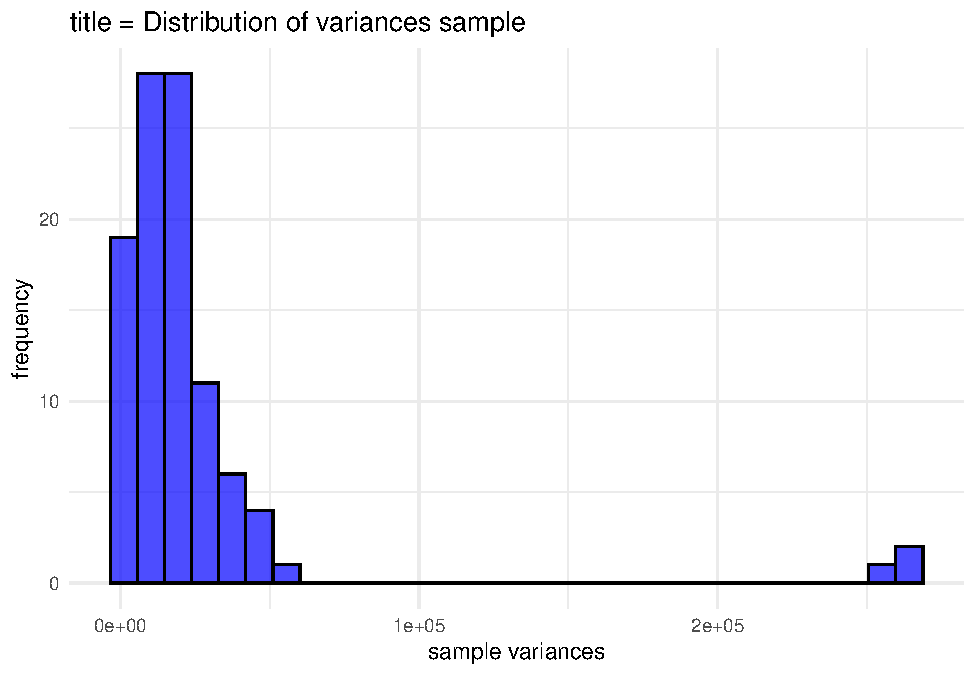
\includegraphics[keepaspectratio]{Assignment14_files/Assignment14_files/figure-latex/unnamed-chunk-15-1.pdf}}

\textbf{Your Answer:}

the mean of sample\_vars is equal to the population variance of the
movie population, which is approximately 3.05 x 10\^{}16.

The standard deviation of sample\_vars is 5.54 x 10\^{}16

The Histogram is extremely right tailed

\emph{step e}

\textbf{Your Answer:}

no, a sample size of 25 is not sufficient. This is because a single mega
hit amongst those 25 can extremely influence the variance of the sample

\textbf{Your answer here}

\section{Week 3}\label{week-3}

For the next part of the assignment, assume that the movies in your data
frame are a random sample of a larger population of movies.

1

\begin{enumerate}
\def\labelenumi{\alph{enumi}.}
\tightlist
\item
  Create a new data set that only includes movies that are of the genre
  ``Thriller''. For these thriller movies, give a 99 percent confidence
  interval for the variable \emph{runtime}. Interpret the result.
  \textbf{[2 points]}
\item
  Now, assume that the variance of \emph{runtime} amongst thriller
  movies in your data is exactly the same as the variance of
  \emph{runtime} in the population. Under this assumption, give a 99
  percent confidence interval for the variable \emph{runtime} among
  thriller movies. Interpret the result. Is you confidence interval
  wider or less wide than the one you found under question 1a? Why is
  that the case? \textbf{[2 points]}
\end{enumerate}

\emph{step a}

\begin{Shaded}
\begin{Highlighting}[]
\NormalTok{thrillers }\OtherTok{\textless{}{-}} \FunctionTok{subset}\NormalTok{(movies1, genre }\SpecialCharTok{==} \StringTok{"Thriller"}\NormalTok{)}
\NormalTok{xbar  }\OtherTok{\textless{}{-}} \FunctionTok{mean}\NormalTok{(thrillers}\SpecialCharTok{$}\NormalTok{runtime, }\AttributeTok{na.rm =} \ConstantTok{TRUE}\NormalTok{)}
\NormalTok{s     }\OtherTok{\textless{}{-}} \FunctionTok{sd}\NormalTok{(thrillers}\SpecialCharTok{$}\NormalTok{runtime, }\AttributeTok{na.rm =} \ConstantTok{TRUE}\NormalTok{)}
\NormalTok{n     }\OtherTok{\textless{}{-}} \FunctionTok{sum}\NormalTok{(}\SpecialCharTok{!}\FunctionTok{is.na}\NormalTok{(thrillers}\SpecialCharTok{$}\NormalTok{runtime))}
\NormalTok{se    }\OtherTok{\textless{}{-}}\NormalTok{ s }\SpecialCharTok{/} \FunctionTok{sqrt}\NormalTok{(n)}
\NormalTok{tcrit }\OtherTok{\textless{}{-}} \FunctionTok{qt}\NormalTok{(}\FloatTok{0.995}\NormalTok{, }\AttributeTok{df =}\NormalTok{ n }\SpecialCharTok{{-}} \DecValTok{1}\NormalTok{)}
\FunctionTok{c}\NormalTok{(xbar }\SpecialCharTok{{-}}\NormalTok{ tcrit }\SpecialCharTok{*}\NormalTok{ se, xbar }\SpecialCharTok{+}\NormalTok{ tcrit }\SpecialCharTok{*}\NormalTok{ se)}
\end{Highlighting}
\end{Shaded}

\begin{verbatim}
## [1]  99.94343 111.01042
\end{verbatim}

\textbf{Your Answer:}

We're 99\% confident the true mean runtime of all thriller movies lies
between 99.94 and 111.01 minutes.

\emph{step b}

\begin{Shaded}
\begin{Highlighting}[]
\NormalTok{zcrit }\OtherTok{\textless{}{-}} \FunctionTok{qnorm}\NormalTok{(}\FloatTok{0.995}\NormalTok{)}
\FunctionTok{c}\NormalTok{(xbar }\SpecialCharTok{{-}}\NormalTok{ zcrit }\SpecialCharTok{*}\NormalTok{ se, xbar }\SpecialCharTok{+}\NormalTok{ zcrit }\SpecialCharTok{*}\NormalTok{ se)}
\end{Highlighting}
\end{Shaded}

\begin{verbatim}
## [1] 100.1081 110.8457
\end{verbatim}

\textbf{Your Answer:}

The 99\% confidence interval is {[}100.11, 110.85{]}. It is narrower
than in part a. This is because we now assume the population variance is
known, so we use the z (normal) distribution instead of the t
distribution. Its critical value is smaller, which gives a narrower
interval.

2

\begin{enumerate}
\def\labelenumi{\alph{enumi}.}
\tightlist
\item
  Using an appropriate five-step procedure, set up a test for the null
  hypothesis that the variance of runtime equals \(500\). Clearly state
  your null hypothesis, alternative hypothesis your test statistic, your
  critical value, and your conclusion. \textbf{[2 points]}
\item
  For the validity of your test in 2a, what assumption about the
  distribution of runtime needs to hold? Make an appropriate plot to
  test this assumption. What do you conclude? \textbf{[2 points]}
\end{enumerate}

\emph{step a}

\begin{Shaded}
\begin{Highlighting}[]
\NormalTok{x  }\OtherTok{\textless{}{-}} \FunctionTok{na.omit}\NormalTok{(movies1}\SpecialCharTok{$}\NormalTok{runtime)}
\NormalTok{n  }\OtherTok{\textless{}{-}} \FunctionTok{length}\NormalTok{(x)}
\NormalTok{s2 }\OtherTok{\textless{}{-}} \FunctionTok{var}\NormalTok{(x)}
\NormalTok{chi2 }\OtherTok{\textless{}{-}}\NormalTok{ (n }\SpecialCharTok{{-}} \DecValTok{1}\NormalTok{) }\SpecialCharTok{*}\NormalTok{ s2 }\SpecialCharTok{/} \DecValTok{500}
\NormalTok{crit }\OtherTok{\textless{}{-}} \FunctionTok{qchisq}\NormalTok{(}\FunctionTok{c}\NormalTok{(}\FloatTok{0.025}\NormalTok{, }\FloatTok{0.975}\NormalTok{), }\AttributeTok{df =}\NormalTok{ n }\SpecialCharTok{{-}} \DecValTok{1}\NormalTok{)}
\NormalTok{pval }\OtherTok{\textless{}{-}} \DecValTok{2} \SpecialCharTok{*} \FunctionTok{min}\NormalTok{(}\FunctionTok{pchisq}\NormalTok{(chi2, n }\SpecialCharTok{{-}} \DecValTok{1}\NormalTok{), }\DecValTok{1} \SpecialCharTok{{-}} \FunctionTok{pchisq}\NormalTok{(chi2, n }\SpecialCharTok{{-}} \DecValTok{1}\NormalTok{))}
\FunctionTok{round}\NormalTok{(}\FunctionTok{c}\NormalTok{(}\AttributeTok{n =}\NormalTok{ n, }\AttributeTok{s2 =}\NormalTok{ s2, }\AttributeTok{chi2 =}\NormalTok{ chi2, }\AttributeTok{crit\_low =}\NormalTok{ crit[}\DecValTok{1}\NormalTok{], }\AttributeTok{crit\_high =}\NormalTok{ crit[}\DecValTok{2}\NormalTok{], }\AttributeTok{p =}\NormalTok{ pval), }\DecValTok{3}\NormalTok{)}
\end{Highlighting}
\end{Shaded}

\begin{verbatim}
##         n        s2      chi2  crit_low crit_high         p 
##   504.000   483.097   485.996   442.750   567.037     0.602
\end{verbatim}

\begin{enumerate}
\def\labelenumi{\arabic{enumi}.}
\tightlist
\item
  \textbf{Hypotheses:} \(H_0: \sigma^2 = 500\) versus
  \(H_1: \sigma^2 \neq 500\) (two-sided).
\item
  \textbf{Significance level:} \(\alpha = 0.05\).
\item
  \textbf{Test statistic:} \(\chi^2 = (n-1)s^2/\sigma_0^2\), which under
  \(H_0\) follows a \(\chi^2\) distribution with \(n-1 = 503\) degrees
  of freedom. With \(n = 504\) movies (one has a missing runtime) and
  \(s^2 = 483.10\), we get \(\chi^2 = 503 \cdot 483.10/500 = 486.00\).
\item
  \textbf{Critical values:} reject \(H_0\) if \(\chi^2 < 442.75\) or
  \(\chi^2 > 567.04\).
\item
  \textbf{Conclusion:} \(\chi^2 = 486.00\) lies between the two critical
  values (p = 0.60), so we do not reject \(H_0\). At the 5\% level there
  is no evidence that the population variance of runtime differs from
  500.
\end{enumerate}

\emph{step b}

\begin{Shaded}
\begin{Highlighting}[]
\FunctionTok{par}\NormalTok{(}\AttributeTok{mfrow =} \FunctionTok{c}\NormalTok{(}\DecValTok{1}\NormalTok{, }\DecValTok{2}\NormalTok{))}
\FunctionTok{hist}\NormalTok{(x, }\AttributeTok{breaks =} \DecValTok{40}\NormalTok{, }\AttributeTok{freq =} \ConstantTok{FALSE}\NormalTok{, }\AttributeTok{main =} \StringTok{"Histogram of runtime"}\NormalTok{,}
     \AttributeTok{xlab =} \StringTok{"Runtime (minutes)"}\NormalTok{)}
\FunctionTok{curve}\NormalTok{(}\FunctionTok{dnorm}\NormalTok{(x, }\AttributeTok{mean =} \FunctionTok{mean}\NormalTok{(x), }\AttributeTok{sd =} \FunctionTok{sd}\NormalTok{(x)), }\AttributeTok{add =} \ConstantTok{TRUE}\NormalTok{, }\AttributeTok{col =} \StringTok{"red"}\NormalTok{, }\AttributeTok{lwd =} \DecValTok{2}\NormalTok{)}
\FunctionTok{qqnorm}\NormalTok{(x, }\AttributeTok{main =} \StringTok{"Normal Q{-}Q plot of runtime"}\NormalTok{)}
\FunctionTok{qqline}\NormalTok{(x, }\AttributeTok{col =} \StringTok{"red"}\NormalTok{, }\AttributeTok{lwd =} \DecValTok{2}\NormalTok{)}
\end{Highlighting}
\end{Shaded}

\pandocbounded{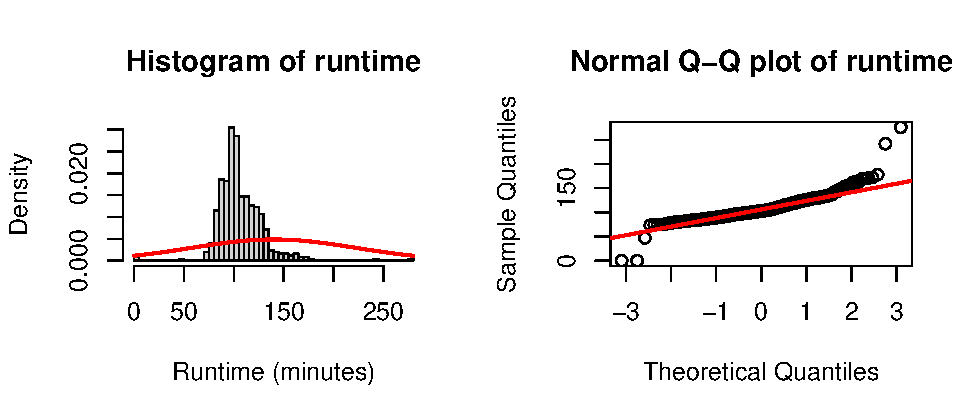
\includegraphics[keepaspectratio]{Assignment14_files/Assignment14_files/figure-latex/unnamed-chunk-19-1.pdf}}

\begin{Shaded}
\begin{Highlighting}[]
\FunctionTok{par}\NormalTok{(}\AttributeTok{mfrow =} \FunctionTok{c}\NormalTok{(}\DecValTok{1}\NormalTok{, }\DecValTok{1}\NormalTok{))}
\end{Highlighting}
\end{Shaded}

\textbf{Your Answer:}

The question says revenue, but the test is about runtime. The \(\chi^2\)
test for a variance is only valid if runtime is normally distributed in
the population, and unlike tests on the mean it stays sensitive to this
even in large samples. The histogram shows that runtime is not normal:
it is right-skewed, with a long upper tail (up to 276 minutes) and a few
values of 0 that look like missing data. In the Q-Q plot the points bend
away from the line in both tails, most clearly in the upper tail. The
normality assumption is therefore violated, so the conclusion in 2a
should be treated with caution.

\begin{enumerate}
\def\labelenumi{\arabic{enumi}.}
\setcounter{enumi}{2}
\tightlist
\item
  There is an argument going on in the movie studio. \emph{Bob} claims
  that they should make higher-quality movies, as this will bring in
  more profits. \emph{Chantal} disagrees. She tells Bob that mediocre
  movies bring in the most profits. You are asked to advise on who is
  right.
\end{enumerate}

\begin{enumerate}
\def\labelenumi{\alph{enumi}.}
\tightlist
\item
  Create a new variable called vote\_average\_rounded. Make sure this
  variable is the same as vote\_average, but without any decimals (i.e.,
  a 6.3 becomes a 6, a 8.7 an 8, etc.). Display a histogram of
  vote\_average\_rounded. \textbf{[2 points]}
\item
  Create a scatter plot with vote\_average\_rounded on the x axis and
  the mean of profits within each category of vote\_average\_rounded on
  the y-axis. Make sure it has an appropriate title, and appropriate
  titles and labels for the x- and y-axis. At which rating of movies are
  profits the highest? \textbf{[3 points]}
\item
  Recreate the scatter plot with year on the x axis and mean\_profits on
  the y-axis, but now add bars around each point, indicating the 95\%
  confidence interval. \textbf{[3 points]}
\item
  Write an advice to settle the argument between Bob and Chantal.
  \textbf{[4 points]}
\end{enumerate}

\emph{step a}

\begin{Shaded}
\begin{Highlighting}[]
\NormalTok{movies1}\SpecialCharTok{$}\NormalTok{vote\_average\_rounded }\OtherTok{\textless{}{-}} \FunctionTok{floor}\NormalTok{(movies1}\SpecialCharTok{$}\NormalTok{vote\_average)}
\FunctionTok{hist}\NormalTok{(movies1}\SpecialCharTok{$}\NormalTok{vote\_average\_rounded, }\AttributeTok{breaks =} \FunctionTok{seq}\NormalTok{(}\SpecialCharTok{{-}}\FloatTok{0.5}\NormalTok{, }\FloatTok{10.5}\NormalTok{, }\AttributeTok{by =} \DecValTok{1}\NormalTok{),}
     \AttributeTok{main =} \StringTok{"Histogram of rounded{-}down vote average"}\NormalTok{,}
     \AttributeTok{xlab =} \StringTok{"Vote average (rounded down)"}\NormalTok{, }\AttributeTok{ylab =} \StringTok{"Number of movies"}\NormalTok{)}
\end{Highlighting}
\end{Shaded}

\pandocbounded{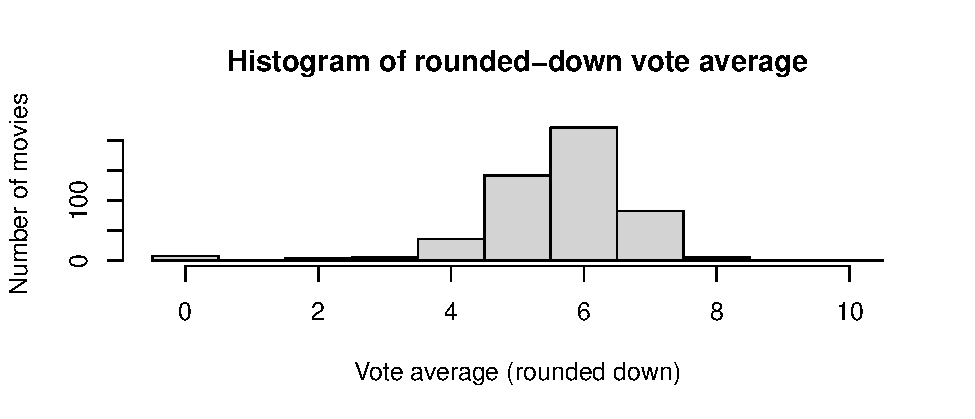
\includegraphics[keepaspectratio]{Assignment14_files/Assignment14_files/figure-latex/unnamed-chunk-20-1.pdf}}

\textbf{Your Answer:}

We use \texttt{floor()}, which drops the decimals (6.7 becomes 6),
rather than \texttt{round()} (which would turn 6.7 into 7). Most movies
have a rating of 5 (142 movies) or 6 (222), followed by 7 (83) and 4
(36). High ratings are rare: only 5 movies score 8 and none score 9 or
10. The 8 movies with a rating of 0 all have zero votes, so their 0 is
really a missing rating.

\emph{step b}

\begin{Shaded}
\begin{Highlighting}[]
\NormalTok{mean\_profits }\OtherTok{\textless{}{-}} \FunctionTok{aggregate}\NormalTok{(profits }\SpecialCharTok{\textasciitilde{}}\NormalTok{ vote\_average\_rounded, }\AttributeTok{data =}\NormalTok{ movies1, }\AttributeTok{FUN =}\NormalTok{ mean)}
\FunctionTok{plot}\NormalTok{(mean\_profits}\SpecialCharTok{$}\NormalTok{vote\_average\_rounded, mean\_profits}\SpecialCharTok{$}\NormalTok{profits }\SpecialCharTok{/} \FloatTok{1e6}\NormalTok{, }\AttributeTok{pch =} \DecValTok{19}\NormalTok{,}
     \AttributeTok{main =} \StringTok{"Mean profit by movie rating"}\NormalTok{,}
     \AttributeTok{xlab =} \StringTok{"Vote average (rounded down)"}\NormalTok{, }\AttributeTok{ylab =} \StringTok{"Mean profit (millions of $)"}\NormalTok{)}
\end{Highlighting}
\end{Shaded}

\pandocbounded{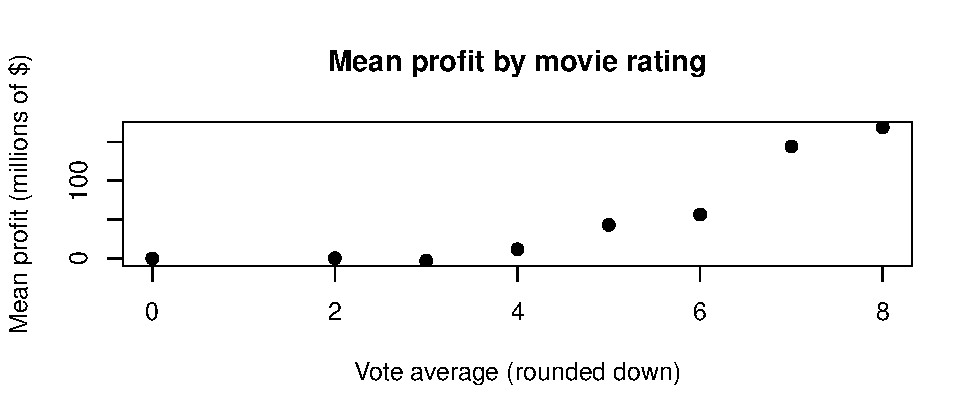
\includegraphics[keepaspectratio]{Assignment14_files/Assignment14_files/figure-latex/unnamed-chunk-21-1.pdf}}

\textbf{Your Answer:}

Mean profits are highest for movies rated 8, at about \$168.7 million,
followed by movies rated 7 (\$144.1 million). Profits rise steadily with
the rating: movies rated 5 and 6 make on average \$43.1 and \$56.5
million, and movies rated 4 or lower make close to nothing.

\emph{step c}

\begin{Shaded}
\begin{Highlighting}[]
\NormalTok{ci }\OtherTok{\textless{}{-}} \FunctionTok{do.call}\NormalTok{(data.frame, }\FunctionTok{aggregate}\NormalTok{(profits }\SpecialCharTok{\textasciitilde{}}\NormalTok{ vote\_average\_rounded, }\AttributeTok{data =}\NormalTok{ movies1,}
        \AttributeTok{FUN =} \ControlFlowTok{function}\NormalTok{(v) }\FunctionTok{c}\NormalTok{(}\AttributeTok{mean =} \FunctionTok{mean}\NormalTok{(v), }\AttributeTok{sd =} \FunctionTok{sd}\NormalTok{(v), }\AttributeTok{n =} \FunctionTok{length}\NormalTok{(v))))}
\FunctionTok{names}\NormalTok{(ci) }\OtherTok{\textless{}{-}} \FunctionTok{c}\NormalTok{(}\StringTok{"rating"}\NormalTok{, }\StringTok{"mean"}\NormalTok{, }\StringTok{"sd"}\NormalTok{, }\StringTok{"n"}\NormalTok{)}
\NormalTok{ci}\SpecialCharTok{$}\NormalTok{lower }\OtherTok{\textless{}{-}}\NormalTok{ (ci}\SpecialCharTok{$}\NormalTok{mean }\SpecialCharTok{{-}} \FunctionTok{qt}\NormalTok{(}\FloatTok{0.975}\NormalTok{, ci}\SpecialCharTok{$}\NormalTok{n }\SpecialCharTok{{-}} \DecValTok{1}\NormalTok{) }\SpecialCharTok{*}\NormalTok{ ci}\SpecialCharTok{$}\NormalTok{sd }\SpecialCharTok{/} \FunctionTok{sqrt}\NormalTok{(ci}\SpecialCharTok{$}\NormalTok{n)) }\SpecialCharTok{/} \FloatTok{1e6}
\NormalTok{ci}\SpecialCharTok{$}\NormalTok{upper }\OtherTok{\textless{}{-}}\NormalTok{ (ci}\SpecialCharTok{$}\NormalTok{mean }\SpecialCharTok{+} \FunctionTok{qt}\NormalTok{(}\FloatTok{0.975}\NormalTok{, ci}\SpecialCharTok{$}\NormalTok{n }\SpecialCharTok{{-}} \DecValTok{1}\NormalTok{) }\SpecialCharTok{*}\NormalTok{ ci}\SpecialCharTok{$}\NormalTok{sd }\SpecialCharTok{/} \FunctionTok{sqrt}\NormalTok{(ci}\SpecialCharTok{$}\NormalTok{n)) }\SpecialCharTok{/} \FloatTok{1e6}
\NormalTok{ci}\SpecialCharTok{$}\NormalTok{mean  }\OtherTok{\textless{}{-}}\NormalTok{ ci}\SpecialCharTok{$}\NormalTok{mean }\SpecialCharTok{/} \FloatTok{1e6}
\FunctionTok{plot}\NormalTok{(ci}\SpecialCharTok{$}\NormalTok{rating, ci}\SpecialCharTok{$}\NormalTok{mean, }\AttributeTok{pch =} \DecValTok{19}\NormalTok{, }\AttributeTok{ylim =} \FunctionTok{range}\NormalTok{(}\FunctionTok{c}\NormalTok{(ci}\SpecialCharTok{$}\NormalTok{lower, ci}\SpecialCharTok{$}\NormalTok{upper)),}
     \AttributeTok{main =} \StringTok{"Mean profit by movie rating with 95\% confidence intervals"}\NormalTok{,}
     \AttributeTok{xlab =} \StringTok{"Vote average (rounded down)"}\NormalTok{, }\AttributeTok{ylab =} \StringTok{"Mean profit (millions of $)"}\NormalTok{)}
\FunctionTok{arrows}\NormalTok{(ci}\SpecialCharTok{$}\NormalTok{rating, ci}\SpecialCharTok{$}\NormalTok{lower, ci}\SpecialCharTok{$}\NormalTok{rating, ci}\SpecialCharTok{$}\NormalTok{upper, }\AttributeTok{angle =} \DecValTok{90}\NormalTok{, }\AttributeTok{code =} \DecValTok{3}\NormalTok{, }\AttributeTok{length =} \FloatTok{0.05}\NormalTok{)}
\end{Highlighting}
\end{Shaded}

\pandocbounded{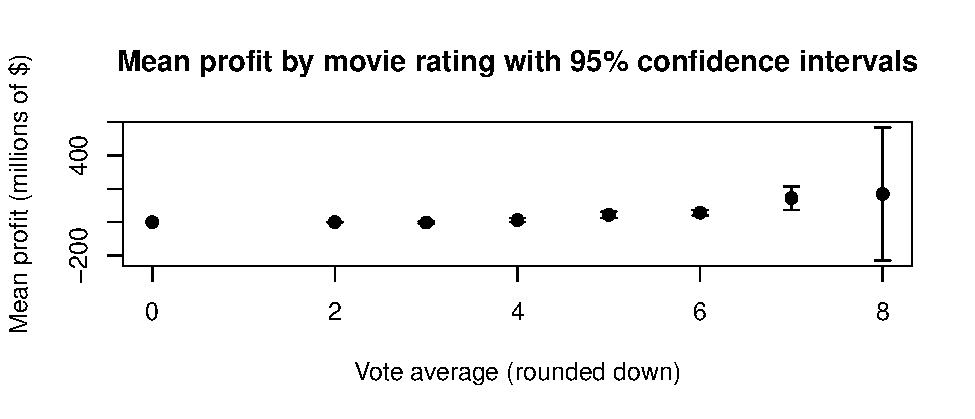
\includegraphics[keepaspectratio]{Assignment14_files/Assignment14_files/figure-latex/unnamed-chunk-22-1.pdf}}

\begin{Shaded}
\begin{Highlighting}[]
\FunctionTok{round}\NormalTok{(ci[, }\FunctionTok{c}\NormalTok{(}\StringTok{"rating"}\NormalTok{, }\StringTok{"n"}\NormalTok{, }\StringTok{"mean"}\NormalTok{, }\StringTok{"lower"}\NormalTok{, }\StringTok{"upper"}\NormalTok{)], }\DecValTok{1}\NormalTok{)}
\end{Highlighting}
\end{Shaded}

\begin{verbatim}
##   rating   n  mean  lower upper
## 1      0   8   0.0    0.0   0.0
## 2      2   4   0.2   -1.1   1.6
## 3      3   5  -2.9   -8.7   3.0
## 4      4  36  11.8   -0.3  23.9
## 5      5 142  43.1   23.7  62.6
## 6      6 222  56.5   40.1  72.9
## 7      7  83 144.1   72.9 215.3
## 8      8   5 168.7 -231.6 569.1
\end{verbatim}

\textbf{Your Answer:}

We interpret ``year'' in the question as vote\_average\_rounded, since
the question asks to recreate the plot from 3b. The intervals are narrow
for ratings 5 and 6 (\$23.7--62.6 million and \$40.1--72.9 million),
where there are many movies. For rating 7 the interval is \$72.9--215.3
million, which lies entirely above the intervals of ratings 5 and 6. The
interval for rating 8 is extremely wide (--\$231.6 to \$569.1 million)
because it is based on only 5 movies, so its high mean is very
uncertain.

\emph{step d}

\textbf{Your Answer:}

The data support Bob rather than Chantal. Mediocre movies (ratings 5--6)
earn on average \$43--56 million, while good movies rated 7 earn about
\$144 million, and the 95\% confidence intervals of these groups do not
overlap. Movies rated 8 have the highest mean profit, but with only 5
such movies this estimate is too uncertain to rely on. There is no
evidence that mediocre movies are the most profitable.

We would still add two caveats. First, this is a correlation, not proof
that quality causes profit: better-rated movies may also have bigger
budgets, famous casts, franchises or more marketing, and popular movies
may attract higher ratings rather than the other way around. Second,
many movies in the data have a budget or revenue of 0, which is probably
missing data and distorts the profit figures. Our advice is that the
studio should aim for well-received (7+) movies, and confirm the effect
of quality with an analysis that controls for budget and genre.

\begin{Shaded}
\begin{Highlighting}[]
\FunctionTok{library}\NormalTok{(tinytex)}
\FunctionTok{library}\NormalTok{(knitr)}
\end{Highlighting}
\end{Shaded}

\section{Week 4}\label{week-4}

\begin{enumerate}
\def\labelenumi{\arabic{enumi}.}
\tightlist
\item
  There is another argument going on in the movie studio. \emph{Bob}
  claims that production budgets are getting out of hand, and that the
  studio should focus on making cheaper movies. \emph{Chantal}
  disagrees. She tells Bob that ``Every dollar we spend on movie
  production is more than offset by the increase in movie profits'\,'.
\end{enumerate}

\begin{enumerate}
\def\labelenumi{\alph{enumi}.}
\tightlist
\item
  Set up a regression model to test Chantal's claim, and estimate it.
  That is, estimate:
  \[\text{Profits}_i=\beta_0+\beta_1 \text{Budget}_i +\varepsilon_i.\]
  Print a summary of your estimated model. \textbf{[2 points]}
\item
  What is the estimated value of \(\beta_1\) and how do you interpet it?
  \textbf{[2 points]}
\item
  Test for the null hypothesis that \(\beta_1 \geq 0\). Report the
  p-value and state your conclusion. \textbf{[2 points]}
\item
  Next, estimate the model
  \[\text{Log Profits}_i=\beta_0+\beta_1 \text{Log Budget}_i +\varepsilon_i.\]
  When creating the variables Log Profits and Log Budget, make sure that
  movies with a Revenue or Budget of zero are assigned the value ``NA''.
  Print a summary of your estimated model \textbf{[2 points]}
\item
  What is the estimated value of \(\beta_1\) and how do you interpet it?
  \textbf{[2 points]}
\item
  Which model has better fit? The level-level model or the log-log
  model? Explain. \textbf{[2 points]}
\item
  Who do you think is correct? Bob or Chantal? What would you advise the
  movie studio to do? \textbf{[2 points]}
\end{enumerate}

\emph{step a}

\begin{Shaded}
\begin{Highlighting}[]
\CommentTok{\#WRITE YOUR CODE HERE}
\end{Highlighting}
\end{Shaded}

\textbf{Your Answer:}

Write your formulated response here.

\emph{step b}

\begin{Shaded}
\begin{Highlighting}[]
\CommentTok{\#WRITE YOUR CODE HERE}
\end{Highlighting}
\end{Shaded}

\textbf{Your Answer:}

Write your formulated response here.

\emph{step c}

\begin{Shaded}
\begin{Highlighting}[]
\CommentTok{\#WRITE YOUR CODE HERE}
\end{Highlighting}
\end{Shaded}

\textbf{Your Answer:}

Write your formulated response here.

\emph{step d}

\begin{Shaded}
\begin{Highlighting}[]
\CommentTok{\#WRITE YOUR CODE HERE}
\end{Highlighting}
\end{Shaded}

\textbf{Your Answer:}

Write your formulated response here.

\emph{step e}

\begin{Shaded}
\begin{Highlighting}[]
\CommentTok{\#WRITE YOUR CODE HERE}
\end{Highlighting}
\end{Shaded}

\textbf{Your Answer:}

Write your formulated response here.

\emph{step f}

\begin{Shaded}
\begin{Highlighting}[]
\CommentTok{\#WRITE YOUR CODE HERE}
\end{Highlighting}
\end{Shaded}

\textbf{Your Answer:}

Write your formulated response here.

\emph{step g}

\begin{Shaded}
\begin{Highlighting}[]
\CommentTok{\#WRITE YOUR CODE HERE}
\end{Highlighting}
\end{Shaded}

\textbf{Your Answer:}

Write your formulated response here.

2

\begin{enumerate}
\def\labelenumi{\alph{enumi}.}
\tightlist
\item
  Make a plot with a 95\% confidence interval with the mean log of
  budget on the y-axis, and whether the first actor of the movie is male
  or female on the x-axis. What do you conclude? \textbf{[2 points]}
\item
  Estimate the following simple OLS model:
  \(log(budget)_i=\beta_0+\beta_1 \text(FirstActorMale)_i + \varepsilon_i.\)
  Is the estimated coefficient for \(\beta_1\) significantly different
  from zero? How do you interpret its estimate, and how does this relate
  to your conclusion in 2a? \textbf{[2 points]}
\item
  Now, have a close look at your data frame. Can you find any instances
  of male first actors who are wrongly labeled as being female, or vice
  versa? What would such mislabelling mean for the coefficient you
  estimated under 2b? \textbf{[2 points]}
\end{enumerate}

\emph{step a}

\begin{Shaded}
\begin{Highlighting}[]
\CommentTok{\#WRITE YOUR CODE HERE}
\end{Highlighting}
\end{Shaded}

\textbf{Your Answer:}

Write your formulated response here.

\emph{step b}

\begin{Shaded}
\begin{Highlighting}[]
\CommentTok{\#WRITE YOUR CODE HERE}
\end{Highlighting}
\end{Shaded}

\textbf{Your Answer:}

Write your formulated response here.

\emph{step c}

\begin{Shaded}
\begin{Highlighting}[]
\CommentTok{\#WRITE YOUR CODE HERE}
\end{Highlighting}
\end{Shaded}

\textbf{Your Answer:}

Write your formulated response here.

\section{Week 5}\label{week-5}

\begin{enumerate}
\def\labelenumi{\alph{enumi}.}
\item
  Create a plot of the mean profits by month of release. Do you see any
  indication that month of release matters to the profits of the movie?
  \textbf{[2 points]}
\item
  Estimate an OLS model which has as dependent variable the log of
  profits of a movie, and as independent variable the log of budget, a
  dummy for whether the movie was released in english or not, and a
  linear term for the month of release. Show a summary of the resulting
  model and interpret each coefficient. \textbf{[4 points]}
\item
  Test for the hypothesis that the coefficient that belongs to month of
  release is zero. \textbf{[2 points]}
\item
  Based on your plot in a.) do you consider the choice that month of
  release enters the model linearly under b.) reasonable? Estimate a
  specification that allows for a more flexible curve. In this new
  specification, test for the null hypothesis that month of release does
  not impact profits. This might require testing multiple terms at once.
  \textbf{[4 points]}
\item
  One executive at the studio wants to time the release of the movie to
  a specific month of the year such that they can maximize revenue.
  Based on your model under d.), What would you advise the movie studio
  regarding the timing of the release of the movie? \textbf{[2 points]}
\end{enumerate}

The movie studio that you work at is releasing a new movie in 2026. It
will be an English-spoken Thriller movie with a budget of 40,000,0000.

\begin{enumerate}
\def\labelenumi{\alph{enumi}.}
\setcounter{enumi}{5}
\tightlist
\item
  Estimate a model that is able to predict the revenue of this movie.
  Give its predicted revenue and include a 99\% prediction interval.
  \textbf{[6 points]}
\end{enumerate}

\emph{step a}

\begin{Shaded}
\begin{Highlighting}[]
\CommentTok{\#WRITE YOUR CODE HERE}
\end{Highlighting}
\end{Shaded}

\textbf{Your Answer:}

Write your formulated response here.

\emph{step b}

\begin{Shaded}
\begin{Highlighting}[]
\CommentTok{\#WRITE YOUR CODE HERE}
\end{Highlighting}
\end{Shaded}

\textbf{Your Answer:}

Write your formulated response here.

\emph{step c}

\begin{Shaded}
\begin{Highlighting}[]
\CommentTok{\#WRITE YOUR CODE HERE}
\end{Highlighting}
\end{Shaded}

\textbf{Your Answer:}

Write your formulated response here.

\emph{step d}

\begin{Shaded}
\begin{Highlighting}[]
\CommentTok{\#WRITE YOUR CODE HERE}
\end{Highlighting}
\end{Shaded}

\textbf{Your Answer:}

Write your formulated response here.

\emph{step e}

\begin{Shaded}
\begin{Highlighting}[]
\CommentTok{\#WRITE YOUR CODE HERE}
\end{Highlighting}
\end{Shaded}

\textbf{Your Answer:}

Write your formulated response here.

\emph{step f}

\begin{Shaded}
\begin{Highlighting}[]
\CommentTok{\#WRITE YOUR CODE HERE}
\end{Highlighting}
\end{Shaded}


\end{document}
